\documentclass[a4paper,12pt]{article}
\usepackage[utf8]{inputenc} %esto mepermite escribir caraceteres acentuados
\usepackage[spanish]{babel} %agrega términos en castellano y separaciòn de palabras
%datos en general
\usepackage{amsmath}
\usepackage{graphicx}

\title{Resumen ORGA I}
\author{Diaz Julian Lautaro}
\date{\today}

\begin{document}

\maketitle

\tableofcontents
\newpage

\section{Introducción}

\begin{itemize}
  \item Arquitectura del computador: atributos visibles al programador(interfaz).
  \begin{itemize}
    \item Set de registros internos.
    \item Set de instrucciones.
    \item Bits utilizados para representar los datos.
    \item Mecanismos de direccionamiento de memoria.
    \item Acceso a dispositivos de entrada y salida.
    \item ...
  \end{itemize}
  \item Organización del computador: cómo se implementa la arquitectura(implementación).
  \begin{itemize}
    \item Señales de control.
    \item Tecnologías de la memoria.
    \item ...
  \end{itemize}
\end{itemize}

\section{Sistemas de representación}
Conjunto de símbolos y reglas que permiten representar los números.

\subsection{Representación de enteros}
\begin{itemize}
  \item Sin signo: todos los bits representan la magnitud y se pueden representar los números en el rango $[0, r^d-1]$, con
  r la base y d la cantidad de dígitos.
  \item Signo+Magnitud: el primer bit se utiliza para indicar el signo (1 negativo, 0 positivo) y el resto para la magnitud.
  N bits pueden representar los números en el rango $[-2^{N-1}-1, 2^{N-1}-1]$.
  \item Complemento a 1: dado un número n en base r con d dígitos, el complementos a 1 se define como $(r^d -1)-n$. Se calcula
  negando todos los bits. N bits pueden representar los números en el rango $[-2^N-1, 2^N-1]$.
  \item Complemento a 2: dado un número n en base r con d dígitos, el complemento a 2 se define como $r^d-n$. Se calcula
  negando todos los bits y sumando 1. N bits pueden representar los números en el rango $[-2^N, 2^N-1]$.
  \item Exceso a m: dado un número n se representa como $n+m$.
\end{itemize}

\subsection{Representación de reales}





\section{Lógica Digital}
\begin{itemize}
\item Compuerta: dispositivo electrónico que produce un resultado en base a un conjunto de valores de entrada.
\item Circuitos: combinación de compuertas que implementan una función booleana. Se dividen en:
\begin{itemize}
  \item Combinatorios: dependen únicamente de la entrada.
  \item Secuenciales: dependen de la entrada y del estado actual.
\end{itemize}
\item Conjunto Universal: un conjunto universal es aquel conjunto de compuerta/s que puede/n construir cualquier circuito
utilizando únicamente a éstas.
\end{itemize}

\subsection{Clock}
Los circuitos secuenciales pueden ser asincrónicos o sincrónicos. Los asincrónicos pueden cambiar su estado en cualquier
momento en el que se modifique su entrada, los asincrónicos utilizan un reloj para ordenar los eventos.
Un clock es un circuito que emite una serie de pulsos con un ancho y un intervalo entre pulsos consecutivos determinado.
Este intervalo se llama ciclo de clock y está dividido en flanco ascendente y descendente. El clock es utilizado por un
circuito secuencial sincrónico para saber cuando los valores de entrada van a modificar su estado.

\subsection{Flip-Flops}
Un flip-flop es un circuito secuencial retroalimentado, lo que permite almacenar bits. Se puede describir el
comportamiento de un flip-flop a través de una tabla característica, que muestra cual va a ser el siguiente estado
basado en las entradas y en el estado actual. Ejemplos de flip-flops son el flip-flop D, SR y JK. Este último es
universal, ya que puede utilizarse para armar los otros dos.





\section{Arquitectura}
Todas las computadoras tienen un CPU (Central Processing Unit). Esta unidad se divide en dos partes. La primera es el
datapath que es una red de unidades de almacenamiento (registros) y unidades lógicas y aritméticas (para realizar
operaciones sobre los datos) conectadas a través de buses (cables que permiten enviar información) donde la
sincronización es controlada por clocks. La segunda parte es la UC (Control Unit), un módulo responsable de ejecutar
operaciones y asegurarse de que los datos sean correctos y estén donde tengan que estar y en el tiempo correcto. Juntos,
estos componentes realizan las tareas del CPU: obtener las instrucciones, decodificarlas y finalmente ejecutar la
secuencia indicada de operaciones.

\subsection{Memoria}
La memoria puede pensarse como una matríz de bits. Cada fila, implementada por un registro, tiene un cierto tamaño. Cada registro (posición en
memoria) tiene una única dirección. Las direcciones suelen representarse con enteros sin signo. Se le llama palabra a la cantidad de bits que
pueden moverse simultáneamente dentro de la CPU (unidad de transferencia). Al tamaño del registro en cada fila se le llama unidad direccionable.

\begin{figure}[ht!]
  \centering
   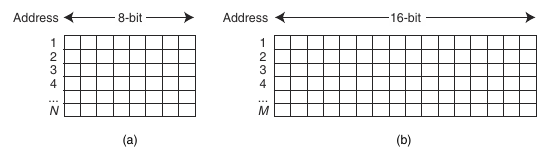
\includegraphics[width=0.6\textwidth]{Imagenes/MEMORIA.png}
  \caption{(a) Memoria de tamaño $8*N-bit$ y unidad direccionable de 8-bit (b) Memoria de tamaño $16*N-bit$ y unidad direccionable de 16-bit}
  \label{MEMORIA}
\end{figure}

\subsection{Unidad de Control}
La unidad de control es la que gestiona el tráfico del CPU. Ésta monitorea la ejecución de todas las instrucciones y
transfiere toda la información, extrayendo la información de la memoria y decodificando las instrucciones, asegurándose
de que los datos estén en el lugar y momento correcto. La UC usa un registro especial llamado PC (Program Counter) para
encontrar la próxima instrucción y, en caso de ser necesario, utiliza registros de estado (flags) para saber en que
estado se encuentra el programa.

\subsection{Ciclo de instrucción}
El ciclo de instrucción representa los pasos que una computadora sigue para correr un programa. Este ciclo tiene 3 etapas:
\begin{enumerate}
  \item Fetch:
  \begin{itemize}
    \item La UC obtiene la próxima instrucción yendo a buscarla a la memoria principal.
    \item La UC incrementa el PC.
  \end{itemize}
  \item Decode: la UC determina el código de operación y carga todos los datos necesarios para llevar a cabo la instrucción.
  \item Execute: la UC realiza la operación indicada por la instrucción.
\end{enumerate}

\subsection{Diseño ISA}
El Instruction Set Architecture (ISA) es el conjunto de instrucciones de una arquitectura. Estas instrucciones se
diferencian por varios aspectos:
\begin{itemize}
  \item Métricas.
  \begin{itemize}
    \item Cantidad total de instrucciones disponibles.
    \item Complejidad del conjunto de instrucciones.
    \begin{itemize}
      \item Reduced Instruction Set Computer (RISC): se simplifican las instrucciones para que se puedan ejecutar más rápido.
      Cada instrucción realiza una única operación, son todas de tamaño fijo y los operandos son únicamente registros.
      \item Complex Instruction Set Computer (CISC): hay una gran cantidad de instrucciones, de longitud variable y un única
      instrucción puede ejecutar múltiples operaciones.
    \end{itemize}
    \item Longitud de las instrucciones.
    \item Cantidad de memoria que un programa requiere.
  \end{itemize}
  \item Tipos de datos soportados.
  \begin{itemize}
    \item Enteros 16/32-bits
    \item Puntos flotante 16/32-bits.
    \item ...
  \end{itemize}
  \item Almacenamiento de los datos.
  \begin{itemize}
    \item ¿Cómo se almacenan los bytes?
    \begin{itemize}
      \item Big Endian: se guardan los bits más significativos primeros.
      \item Little Endian: se guardan los bits menos significativos primeros.
      \begin{figure}[ht!]
        \centering
         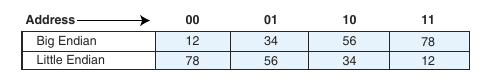
\includegraphics[width=0.6\textwidth]{Imagenes/ENDIAN.png}
        \caption{El valor hexadecimal 12345678 almacenado en Big y Little Endian}
        \label{ENDIAN}
      \end{figure}
    \end{itemize}
    \item ¿Dónde se almacenan?
    \begin{itemize}
      \item Arquitectura de stack: esta arquitectura utiliza una pila para ejecutar instrucciones y los operandos se encuentran al tope
      de ésta.
      \item Arquitectura de acumulador: se tiene un registro especial (AC) que se utiliza como operando implícito.
      \item Arquitectura con registros de propósito general.
      \begin{itemize}
        \item Memoria-Memoria: puede tener muchos operandos en memoria sin recurrir a registros.
        \item Registro-Memoria: operandos en memoria y en registros.
        \item Cargar-Almacenar: operandos únicamente en registros.
      \end{itemize}
    \end{itemize}
    \item ¿Cómo se acceden?
    \begin{itemize}
      \item Inmediato: el valor a ser referenciado sigue inmediatamente al código de operación.
      \item Directo: el valor a ser referenciado se obtiene especificando su
      posición en memoria.
      \item Indirecto: el valor a ser referenciado se obtiene en la posición de memoria contenida en la posición en memoria especificada.
      \item Registro: el valor a ser referenciado se obtiene en el registro especificado.
      \item Indexado: el valor a ser referenciado se obtiene en la posición de memoria resultante de sumar una constante con la posición
      de memoria en el registro especificado.
    \end{itemize}
  \end{itemize}
  \item ¿Qué operaciones puede ejecutar?
  \begin{itemize}
    \item Movimiento de datos.
    \item Aritméticas.
    \item Lógicas.
    \item E/S.
    \item Transferencia de control.
    \item Específicas.
  \end{itemize}
  \item ¿Cómo se codifican las operaciones?
  \begin{itemize}
    \item Código de operación: representa la operación a utilizar.
    \item Fuente/s: información para obtener operandos de origen.
    \item Destino/s: información para obtener la ubicación del resultado de la
    operación.
    \item Referencia a próxima instrucción: información para determinar el próximo valor del PC.
  \end{itemize}

  \begin{figure}[ht!]
    \centering
     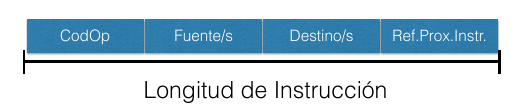
\includegraphics[width=0.6\textwidth]{Imagenes/ISA.png}
    \caption{Modelo de instrucción}
    \label{ISA}
  \end{figure}
\end{itemize}




\subsection{Registros}
Los registros son utilizados para almacenar una amplia variedad de datos como direcciones, contadores o datos necesarios
para la ejecución del programa y son controlados por la UC. Los registros están en el procesador, eso hace que la
información pueda ser accedida rápidamente. Pueden ser implementados usando flip-flops D en paralelo.

\subsection{Unidad Aritmético Lógica}
La Unidad Aritmético Lógica (ALU) lleva a cabo las operaciones lógicas (como comparaciones) y aritméticas (como la suma,
resta o multiplicación) requeridas durante la ejecución del programa. Ésta es controlada, a través de señales que indican
que operación realizar, por la UC.

\subsection{Buses}
La CPU se comunica con los otros componentes a través del bus. Un bus es un conjunto de cables que actúa como una ruta
para conectar múltiples subsistemas dentro del sistema. Éstos pueden conectar únicamente dos dispositivos específicos
(dedicado) o muchos a la vez (multiplexado). En general, los dispositivos se dividen en master y slave, donde el maestro
es aquel que empieza la acción y el esclavo el que responde a ella. Hablamos de escritura cuando el master quiere enviar
datos y de lectura cuando quiere recibirlos. Para evitar escrituras simultáneas es necesario un protocolo de bus y para
esto se utilizan líneas de control que indican que dispositivo tiene permiso para usar el bus y para que propósito. Los
protocolos pueden ser sincrónicos o asincrónicos. Los buses que conectan el procesador con la memoria suelen ser cortos
y rápidos para maximizar el ancho de banda. En cambio, los buses de Entrada/Salida (E/S) son más largos y permiten ser
utilizados por distintos tipos de arquitecturas.

\subsection{Clocks}
Todas las computadoras tienen un clock interno que regula que tan rápido se pueden ejecutar las instrucciones. El clock
regula el ritmo de todo lo que pasa en el sistema. La CPU requiere un determinado número de ciclos de clock para ejecutar
cada instrucción. Algunos buses también tienen su propio clock y éste suele ser más lento que el del CPU.





\section{E/S}
Los dispositivos de E/S nos permiten comunicarnos con la computadora. E/S es la transferencia de datos entre la memoria
primaria y varios periféricos de E/S. Hay una interfaz que maneja la transferencia de datos. Esta interfaz convierte
las señales del bus en un formato reconocible por el dispositivo. La CPU se comunica con estos dispositivos externos
a través de registros específicos de E/S. La interfaz puede mapear los registros a la memoria principal o el dispositivo
puede tener registros propios y la CPU utiliza instrucciones especiales para poder comunicarse. A continuación vemos dos
maneras para controlar la transferencia de información entre CPU y dispositivos de E/S.

\subsection{Interrupciones}
Las interrupciones son eventos que alteran la normal ejecución del programa. El dispositivo de E/S interrumpe a la CPU
cuando quiere comunicarse. En este momento la CPU guarda el estado actual en el que se encontraba antes de la
interrupción y ejecuta la Rutina de Atención de Interrupciones (RAI), un programa que se carga en alguna posición de
memoria. Al finalizar la RAI se vuelve al estado anterior del programa. En la Figura \ref{INTR} se puede ver como puede ser
implementado un sistema para manejar interrupciones. Cuando el dispositivo interrumpe el controlador de interrupciones
activa la señal Interrupt (INT). Cuando la CPU está lista para procesar la interrupción activa la señal Interrupt
Acknowledge (INTA). Luego el controlador puede bajar la señal INT.
\begin{figure}[ht!]
  \centering
   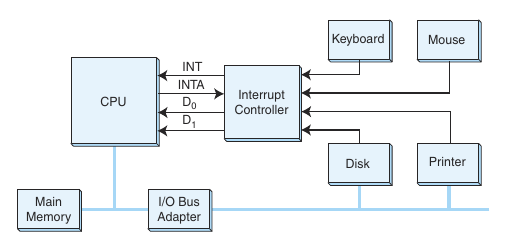
\includegraphics[width=0.6\textwidth]{Imagenes/INTR.png}
  \caption{Modelo de E/S con interrupciones}
  \label{INTR}
\end{figure}

\subsection{Polling}
En este caso, en cada ciclo antes de realizar el fetch, la CPU, a través de un flag, se fija si el dispositivo de E/S
solicitó comunicarse y de ser así interrumpe la ejecución del programa realizando lo mismo que con interrupciones.

\subsection{DMA}
Con polling e interrupciones la CPU mueve datos hacia y desde los dispositivos de E/S. Para alivianar el trabajo de la
CPU se implementa un chip dedicado, llamado Direct Memory Access (DMA), para poder acceder a la memoria sin tener que
recurrir a la CPU. La CPU le envía una señal a la DMA y procede con la siguiente tarea, mientras la DMA se ocupa del
dispositivo de E/S. Cuando finaliza, la DMA envía otra interrupción a la CPU.

\begin{figure}[ht!]
  \centering
   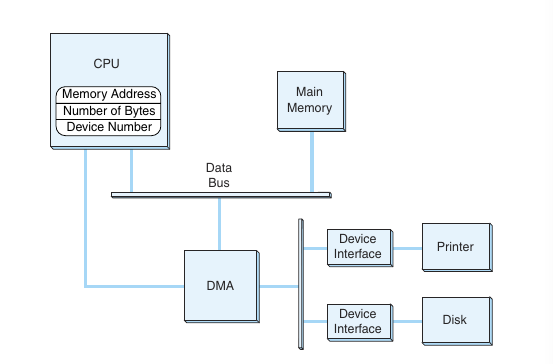
\includegraphics[width=0.6\textwidth]{Imagenes/DMA.png}
  \caption{Modelo de DMA}
  \label{DMA}
\end{figure}





\section{Microarquitectura}
Cada instrucción está compuesta por microinstrucciones. Estas microinstrucciones realizan pasos muy simples, por
ejemplo poner cosas en registros, activar circuitos o prender/apagar líneas. La UC es la encargada de ejecutar
estas microinstrucciones, a través de señales de control. Hay dos maneras de implementar la UC y ambas
tienen señales de tiempo para saber en que paso están. Estas señales se generan con un simple contador. Por ejemplo,
una arquitectura podría incluir las señales de tiempo $T_1,...,T_8$, el fetch de una instrucción podría ocurrir cuando
se active $T_1$ y el fetch de un operando cuando se active $T_4$, etcétera.

\begin{itemize}
  \item UC Cableada (Hardwired): esta UC se implementa utilizando hardware (circuitos). Los circuitos van a tener
  como entradas el código de operación, los flags, señales del bus y señales del clock. Esta UC es muy rápida,
  pero difícil de diseñar y modificar.

  \begin{figure}[ht!]
    \centering
     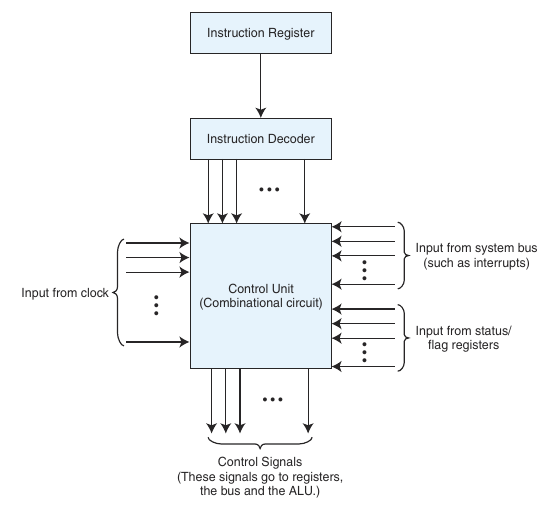
\includegraphics[width=0.6\textwidth]{Imagenes/UC_HARDWIRED.png}
    \caption{Ejemplo de UC cableada}
    \label{UC_HARDWIRED}
  \end{figure}

  \item UC Microprogramada: todas las instrucciones son entradas a un microprograma, que convierte estas instrucciones en señales de
  control. Este microprograma es programa escrito en un lenguaje de bajo nivel que se implementa directamente por hardware.
  Para cada instrucción hay una subrutina y para modificar una instrucción o agregar una nueva alcanza con modificar la subrutina o
  agregar otra. La ventaja de esto es que es flexible (no hace falta modificar el hardware) y simple de diseñar, pero más lenta que la cableada.
  \begin{figure}[ht!]
    \centering
     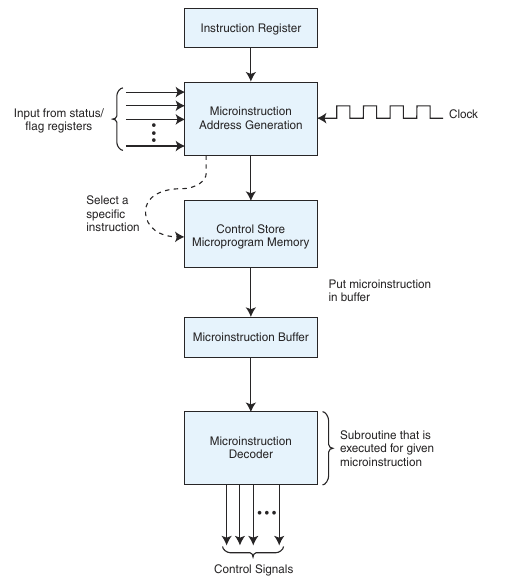
\includegraphics[width=0.6\textwidth]{Imagenes/UC_MICRO.png}
    \caption{Ejemplo de UC microprogramada}
    \label{UC_MICRO}
  \end{figure}
\end{itemize}




\section{Memorias}
Hay dos tipos básicos de memoria:
\begin{itemize}
  \item RAM (Random Access Memory): la memoria RAM es la memoria principal. Se utiliza para almacenar programas
  y datos que la computadora necesita cuando se ejecutan los programas. Esta memoria es volátil, pierde su
  información al cortarse la corriente.
  \begin{itemize}
    \item DRAM (dynamic): construida con pequeños capacitores que pierden electricidad. Necesita una recarga cada
    pocos milisegundos para mantener sus datos. Es más densa y usa menos corriente que la SRAM. Se suele usar
    para la memoria principal.
    \item SRAM (static): construida con circuitos similares a los flip-flops D. Mantiene sus datos mientras tenga
    corriente. Es más rápida, pero más cara que la DRAM. Se suele usar para la memoria caché.
  \end{itemize}
  \item ROM (Read Only Memory): en esta memoria se almacena la información necesaria para usar el sistema, como
  el programa necesaria para arrancar la computadora. La ROM no es volátil, mantiene su información aunque se
  corte la corriente. Este tipo de memoria suele ser utilizada en sistemas encrustados o en cualquier sistema
  donde la información no necesitar modificarse. Se dividen según cuando pueden ser escritas.
  \begin{itemize}
    \item ROM: se escribe una única vez en la fábrica.
    \item PROM (Programable): puede ser escrita por el usuario una única vez.
    \item EPROM (Erasable): puede ser escrita varias veces por el usuario, con luz ultravioleta, eliminando toda
    la información de antemano.
    \item EEPROM (Electrical): puede ser escrita o borrada varias veces de manera electrónica y se borra un byte a la vez.
    \item Memoria Flash: igual a la EEPROM, pero permite borrar de a bloques.
  \end{itemize}
\end{itemize}

\subsection{Jerarquía de memoria}
Vimos que no todas las memorias son creadas de la misma manera, y algunos tipos son menos eficientes y más baratos que otros.
Para tratar esta disparidad, las computadoras utilizan una combinación de tipos de memoria para obtener la mejor relación
precio-eficiencia posible. A este enfoque se le llama jerarquía de memoria. Cuanto más rápida es una memoria, más caro es el
almacenamiento por bit. Los tipos básicos que normalmente constituyen la jerarquía de memoria son los registros, la caché, la
memoria principal y la memoria secundaria. Hoy en día, las computadoras tienen pequeña cantidad de memoria muy rápida, llamada
caché. La caché está conectada a la memoria principal, que es más grande y de mediana rapidez. La memoria principal se
complementa con una memoria secundaria mucho más grande y lenta. Estas memorias las clasificamos según cuantos ciclos le
requieren a la CPU para poder acceder a ellas. A continuación vemos terminología usada cuando hablamos de jerarquía de memoria.
La caché es un tipo de memoria, chica y rápida, que sirve como buffer para un acceso a datos frecuente.





\section{Performance}





\section{Bibliografía}
\begin{itemize}
  \item The Essentials of Computer Organization and Architecture - Linda Null, Julia Lobur
  \item Apuntes $1^{er}$ cuatrimestre 2018
\end{itemize}









\end{document}
